\documentclass[sigconf,screen,review]{acmart}
\settopmatter{printacmref=false}
\setcopyright{none}
\acmConference[WWW Companion '27]{Companion Proceedings of the ACM Web Conference 2027}{May 10--14, 2027}{Dublin, Ireland}
\usepackage{booktabs}
\usepackage{xcolor}
\usepackage{xspace}
% Every \pending{} must be resolved before submission.
\newcommand{\pending}[1]{\textcolor{red}{[PENDING: #1]}}
% Generated by src/paper_numbers.py; do not edit.
\newcommand{\measureDate}{2026-10-21\xspace}
\newcommand{\labDeclared}{571\xspace}
\newcommand{\labEndpoint}{493\xspace}
\newcommand{\labAnswering}{199\xspace}
\newcommand{\labAnsweringPct}{40\xspace}
\newcommand{\labBrowser}{129\xspace}
\newcommand{\labBrowserPctOfAnswering}{65\xspace}
\newcommand{\labBrowserPctOfEndpoint}{26\xspace}
\newcommand{\labConnFail}{134\xspace}
\newcommand{\labTlsFail}{32\xspace}
\newcommand{\labHttpFail}{128\xspace}
\newcommand{\altAnswering}{209\xspace}
\newcommand{\altBrowser}{132\xspace}
\newcommand{\windowedN}{6\xspace}
\newcommand{\labCollected}{158\xspace}
\newcommand{\labLabelsM}{59.1\xspace}
\newcommand{\labPostPct}{81\xspace}
\newcommand{\labAccountPct}{17\xspace}
\newcommand{\labTopFivePct}{66\xspace}
\newcommand{\labInertPct}{10.2\xspace}
\newcommand{\labInertMajority}{20\xspace}
\newcommand{\labRetractedPct}{4.4\xspace}
\newcommand{\latN}{24\xspace}
\newcommand{\latFastN}{9\xspace}
\newcommand{\latSlowN}{10\xspace}
\newcommand{\accProtM}{2.9\xspace}
\newcommand{\accTwoPlusPct}{3.1\xspace}
\newcommand{\lensPostN}{42,454\xspace}
\newcommand{\lensAcctN}{4,640\xspace}
\newcommand{\lensPostProtDiffPct}{42.6\xspace}
\newcommand{\lensPostPopDiffPct}{0.9\xspace}
\newcommand{\lensPostAllDiffPct}{62.8\xspace}
\newcommand{\lensAcctProtDiffPct}{11.5\xspace}
\newcommand{\lensAcctPopDiffPct}{9.2\xspace}
\newcommand{\lensAcctAllDiffPct}{45.9\xspace}
\newcommand{\lensTopDriver}{pef-moderation.org\xspace}
\newcommand{\lensTopDriverPct}{99.7\xspace}
\newcommand{\lensTableRows}{\multicolumn{5}{@{}l}{\emph{Posts (n=42,454)}} \\
    \quad Logged-out visitor & 5.2 & 0.0 & 0.0 & 94.8 \\
    \quad Popular stack & 5.2 & 0.0 & 0.9 & 93.9 \\
    \quad Protective stack & 6.6 & 0.3 & 40.8 & 52.2 \\
    \quad All that labelled it & 10.7 & 12.7 & 44.6 & 32.0 \\
    \multicolumn{5}{@{}l}{\emph{Accounts (n=4,640)}} \\
    \quad Logged-out visitor & 0.0 & 0.0 & 0.0 & 100.0 \\
    \quad Popular stack & 0.0 & 0.5 & 8.8 & 90.8 \\
    \quad Protective stack & 1.1 & 0.8 & 9.7 & 88.5 \\
    \quad All that labelled it & 3.3 & 0.9 & 41.8 & 54.1 \\}
\newcommand{\snapSources}{61\xspace}
\newcommand{\censusTried}{27\xspace}
\newcommand{\censusGone}{7\xspace}
\newcommand{\censusN}{20\xspace}
\newcommand{\censusMedian}{3.2\xspace}
\newcommand{\censusMax}{4.9\xspace}
\newcommand{\censusLive}{118\xspace}
\newcommand{\censusTotalMedian}{15.0\xspace}
\newcommand{\censusRevivedMax}{3\xspace}
\newcommand{\figLabelers}{8\xspace}
\newcommand{\figOutcomes}{3\xspace}
\newcommand{\figDate}{2026-10-21\xspace}
\newcommand{\figAnswered}{186\xspace}
\newcommand{\figSnapshot}{61\xspace}
\newcommand{\figLive}{125\xspace}
\newcommand{\codeLines}{580\xspace}


\begin{document}
\sloppy
\title{LabelLens: Seeing a Bluesky Post Through Other People's Moderation}
\author{Seungbum Ju}
\affiliation{\institution{Samsung Electronics}\city{Seoul}\country{Republic of Korea}}
\email{seungbum.ju@samsung.com}

\begin{abstract}
On Bluesky, moderation is \emph{stackable}: anyone can run a labeling service, and each user chooses which of these \emph{labelers} to trust. Two people can therefore see the same post very differently, and nobody, including its author, sees the whole picture. We present LabelLens, a serverless web tool that asks every public labeler about a post or an account at once and renders the item through several subscription sets with the official client's moderation code, side by side. A companion page reports a network-wide measurement of all \labDeclared declared labelers. Only \labAnswering of their \labEndpoint published endpoints answer queries, and \labBrowserPctOfAnswering\% of those allow a browser to read the answer. In a uniform sample of labelled posts, the twenty most-liked protective labelers change how \lensPostProtDiffPct\% are presented to a subscriber compared with a logged-out visitor, and \lensPostProtHardDiffPct\,pp more are hidden or put behind a warning, mostly because clients apply an author's account labels to their posts. \lensTopDriverPct\% of the changed posts carry a label from a single service; without it the change is \lensPostProtNoTopDiffPct\%. The twenty most-liked labelers overall change \lensPostPopDiffPct\%. LabelLens runs from a link, with no login and no server.

\end{abstract}
\ccsdesc[500]{Information systems~Social networking sites}
\ccsdesc[300]{Human-centered computing~Collaborative and social computing systems and tools}
\keywords{decentralized social media, Bluesky, AT Protocol, content moderation, labeling, transparency}
\maketitle

\section{Introduction}
\label{sec:intro}
Bluesky replaces a single platform moderator with \emph{labels}~\cite{Bluesky_2023,Kleppmann_2024}. A labeler is an account that signs short values such as \texttt{spam} or \texttt{ai-imagery} and attaches them to posts or accounts~\cite{ATProto_labels}. Every client applies Bluesky's own labeler, and a signed-in user may subscribe to up to twenty more and decide, per label, whether to hide, warn or ignore. This realises the long-standing idea of moderation \emph{middleware}~\cite{Hogg_2024}, but it also fragments what people see. An author cannot tell which labels follow their account, a reader cannot tell what other readers are shown, and researchers have so far studied either the network's infrastructure~\cite{Balduf_2024} or Bluesky's own labeler~\cite{Singh_2026}, which explicitly leaves third-party labelers to future work.

LabelLens makes this fragmentation visible for one item at a time. Given a post link or a handle, it (i)~runs a \emph{census}, asking every labeler in a network-wide directory what it says about the post, its author and the author's profile, and (ii)~shows the item through \emph{lenses}, that is, subscription sets evaluated with the moderation code of the official client library. A companion \emph{Network} page summarises a measurement of all labelers. The demonstration offers three things: a tool anyone can run from a link, a census method that copes with a network where most services are unreachable from a browser, and measured evidence of how far the stacks diverge.

\begin{figure*}[t]
  \centering
  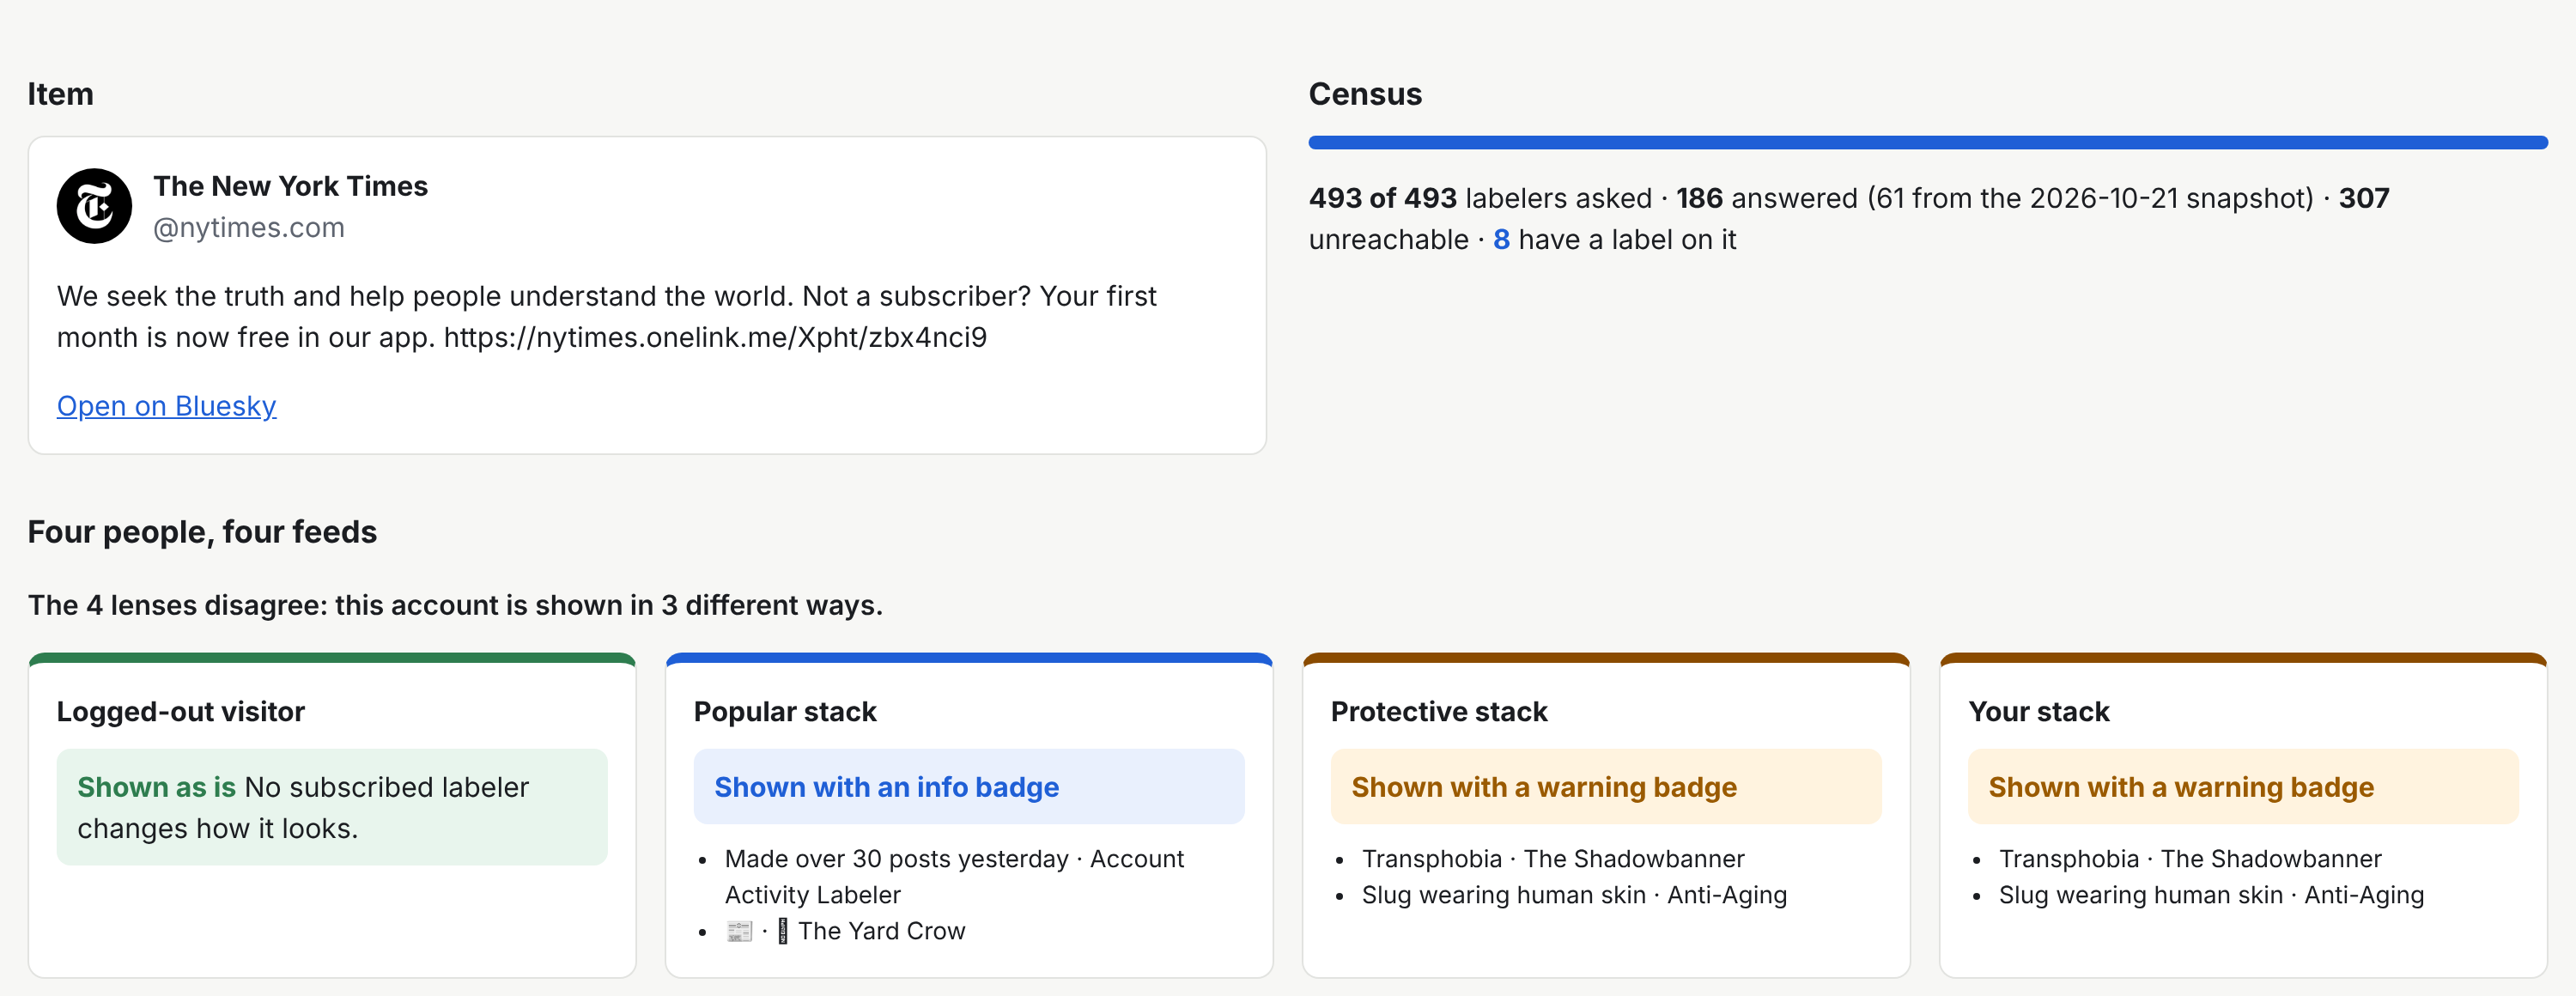
\includegraphics[width=\textwidth]{figures/ui_inspect.png}
  \caption{Inspecting a news organisation's account (\figDate): \figLabelers labelers label it, and the four lenses show it in \figOutcomes different ways. In this run \figAnswered services answered (\figLive live from the browser, \figSnapshot from the snapshot), against \labAnswering endpoints that answered our server-side probe (Section~\ref{sec:eval}). Labels are the labelers' own claims.}
  \label{fig:ui}
  \Description{Screenshot of the LabelLens Inspect page with the item, census progress, four lens cards and the per-labeler list.}
\end{figure*}

\section{LabelLens}
\label{sec:system}
LabelLens is a static site (GitHub Pages) of about \codeLines lines of JavaScript; every request goes from the visitor's browser to public endpoints. Figure~\ref{fig:ui} shows the Inspect view.

\textbf{Directory.} Labelers are ordinary accounts that publish an \texttt{app.bsky.labeler.service} record and a \texttt{\#atproto\_labeler} endpoint in their DID document~\cite{ATProto_labels}. We list the accounts holding such a record through the relay's \texttt{listReposByCollection}, resolve each DID document, and ship the resulting directory (\labEndpoint endpoints) with the site; a GitHub Actions workflow repeats the whole measurement.

\textbf{Census.} For an item, the browser sends one \texttt{queryLabels} request per labeler (32 in parallel) for the post, the author's DID (account labels) and the profile record (only the last two for an account). Each answer is folded into the labels in force now: the latest label per (labeler, subject, value) wins, a negation retracts it, and an expired label is dropped. Only labels whose source is the queried labeler are kept (signatures are not verified), because some services replay other labelers' labels. Many labelers answer but send no CORS header, so a page cannot read them. For the \snapSources services without CORS whose label streams we collected, a snapshot of their labels in force at collection time, sharded into 4{,}096 static files by a hash of the subject's DID, fills the gap, and those rows are marked as snapshot data. The public site ships the snapshot only for its example accounts, so it republishes no labels about individuals; a local build, as used for a live demo, loads all of it. To show the lenses quickly, the census runs in two phases: first the services that answered at our last measurement (4\,s timeout); then those that were offline (4\,s) and those that were slow (8\,s) are retried, and the lenses are recomputed if any of them answers.

\textbf{Lenses.} A lens is a subscription set. LabelLens passes the census result and the labelers' own label definitions, fetched live, to \texttt{moderatePost} or \texttt{moderateProfile} from \texttt{@atproto/api}, with default preferences and adult content off, and reports the decision for a feed or a profile list: hidden, behind a warning, warning badge, info badge, or shown as is, with the labels that caused it. The four lenses are a \emph{logged-out visitor} (Bluesky's labeler only, which is also all the public read API returns), a \emph{popular stack} (the twenty most-liked labelers), a \emph{protective stack} (the twenty most-liked labelers that declare a label that hides, blurs or warns) and \emph{your stack}, which starts from the labelers that labelled the item (at most twenty, the client's limit) and can be edited.

\textbf{Network page.} The measurement of Section~\ref{sec:eval} is published as a sortable table and summary tiles (Figure~\ref{fig:network}): reachability, label volume, retractions, labels without effect and time to label, per service and in aggregate only.


\section{Measurement and Evaluation}
\label{sec:eval}
\textbf{Data.} A GitHub Actions run on \measureDate\ listed the labeler directory, probed every endpoint once, and replayed each labeler's full label stream with \texttt{subscribeLabels} from sequence zero. For the \windowedN services whose stream had passed sequence number three million, only the last three million sequence numbers were replayed. An earlier run from a second vantage point (our cloud workspace) gave nearly the same reachability (\altAnswering answering, \altBrowser browser-readable), so the failures below are the services', not the vantage point's. The author set the topic and the direction of the experiments; an AI assistant (Anthropic Claude) helped carry them out and analyse them.

\textbf{Reachability.} Of \labDeclared accounts that declare a labeler, \labEndpoint publish an endpoint, but only \labAnswering (\labAnsweringPct\%) answer a \texttt{queryLabels} request; the rest cannot be reached (\labConnFail), fail TLS (\labTlsFail) or answer with an HTTP error or a body that is not JSON (\labHttpFail). Of the answering services, \labBrowser (\labBrowserPctOfAnswering\%) send a CORS header. A browser-only client such as a third-party app or LabelLens itself therefore sees at most \labBrowserPctOfEndpoint\% of declared endpoints, which is why the census needs its snapshot fallback.

\begin{figure}[t]
  \centering
  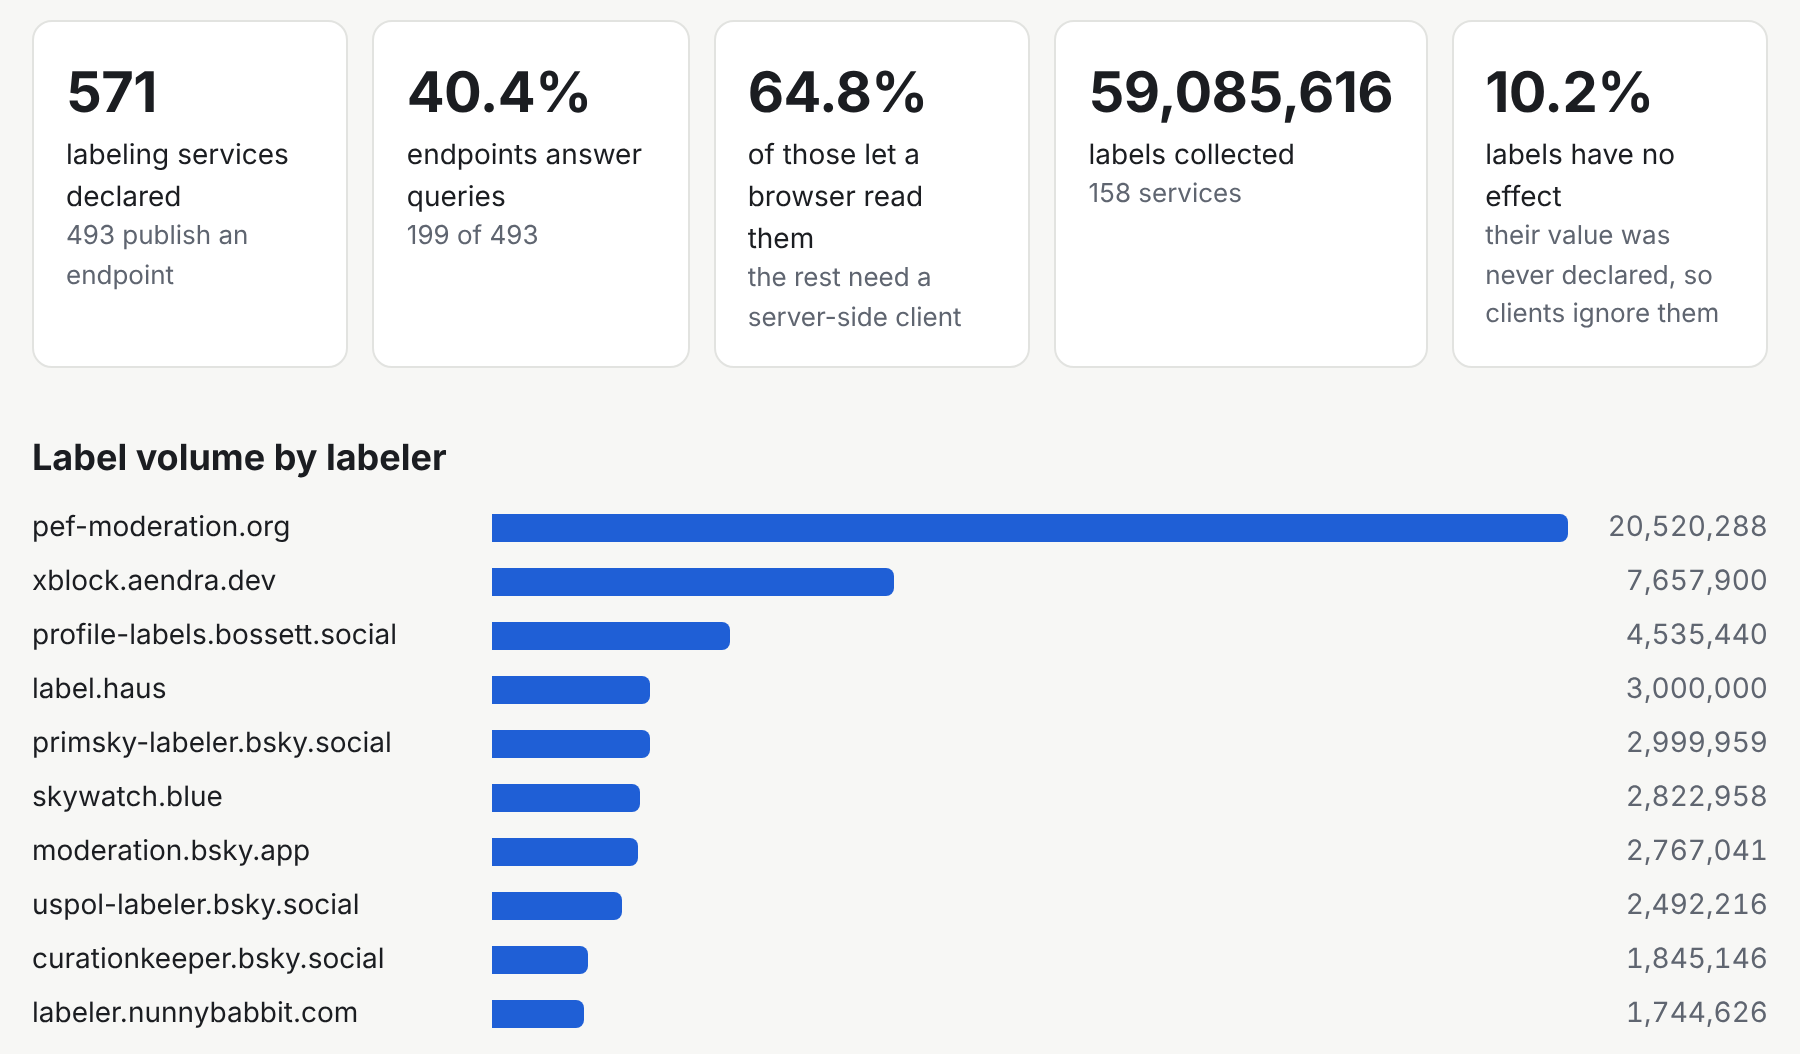
\includegraphics[width=\columnwidth]{figures/ui_network.png}
  \caption{The Network page (\measureDate): summary tiles and the ten services with the most labels. Services whose stream had passed sequence number three million, such as \texttt{moderation.bsky.app}, were replayed from a recent window, so their bars count that window only.}
  \label{fig:network}
  \Description{Five summary tiles (571 labeling services declared, 40.4\% of endpoints answer, 64.8\% of those browser-readable, 59 million labels collected, 10.2\% of labels have no effect) above a horizontal bar chart of label volume for the ten largest labelers.}
\end{figure}

\textbf{Labels.} We collected \labLabelsM million labels from \labCollected services (\labPostPct\% on posts, \labAccountPct\% on accounts). Volume is concentrated: the five largest services issued \labTopFivePct\% of all labels. \labInertPct\% of labels carry a value their labeler never declared; clients drop such labels silently, and for \labInertMajority services they are the majority. \labRetractedPct\% of (subject, value) pairs end retracted. Protective labelers differ widely in speed: among the \latN with at least 100 post labels, the median time from post creation to label is under ten seconds for \latFastN (automated classifiers) and over an hour for \latSlowN.

\textbf{Overlap and divergence.} Stacks rarely agree because they rarely overlap: of the \accProtM million accounts labelled by any protective labeler, \accTwoPlusPct\% are labelled by two or more. To measure what this means for readers, we drew a uniform sample of labelled subjects (a subject is kept when its hash is 0 modulo 1{,}000; \lensPostN posts and \lensAcctN accounts) and evaluated each lens offline with the same moderation code as the site (Table~\ref{tab:lens}). For posts, the protective stack changes the presentation of \lensPostProtDiffPct\% relative to a logged-out visitor, mostly by adding an info badge, while the popular stack changes only \lensPostPopDiffPct\%: the most-liked labelers are mostly descriptive (badges, interests, verification), so popularity is a poor guide to protection. The effect is also concentrated: \lensTopDriverPct\% of the changed posts are changed by one service, \texttt{\lensTopDriver}, which flags links to other platforms and suspected disinformation sources. Which labelers a user adds matters more than how many, and this is exactly what the census and the editable stack expose for a single item. Subscribing to the labelers that labelled the item (at most twenty) changes \lensPostAllDiffPct\% of posts.

\begin{table}[t]
  \caption{How labelled items are shown under each lens (uniform sample; percent of items).}
  \label{tab:lens}
  \small
  \begin{tabular}{@{}lrrrr@{}}
    \toprule
    Lens & Hidden & Warned & Info badge & As is \\
    \midrule
    \lensTableRows
    \bottomrule
  \end{tabular}
\end{table}

\textbf{Census performance.} We tried \censusTried items (posts and accounts from the sample) in headless Chromium from our workspace; \censusGone sampled posts had since been deleted or hidden, and the other \censusN were inspected. The lenses appeared after \censusMedian\,s at the median (\censusMax\,s at most); the recheck of slow services and of those offline at measurement time finished after \censusTotalMedian\,s and added at most \censusRevivedMax answers. At least \censusLive labelers answered live on every run, and \snapSources more through the full snapshot.

\section{Demonstration}
\label{sec:demo}
Visitors open LabelLens at \url{https://seungbum.github.io/labellens/} (no login). A typical walk-through takes three minutes. (1)~Paste a post link or a handle, or click an example; the census bar fills as \labValidEndpoint services are asked. (2)~Compare the four lens cards: the same item may be shown as is to a logged-out visitor, with an info badge in the popular stack and with a warning in the protective stack, each with the labels that caused it. (3)~Open \emph{your stack} and toggle labelers to see which one decides the outcome. (4)~Scan the per-labeler list, where struck-through labels were retracted, faded ones expired, and dashed ones have no effect. (5)~Switch to the Network page to see how few services are reachable and how unevenly labels are spread. At the conference we run the same public build, on our laptop or the attendee's phone: attendees can inspect their own accounts, and for any account other than the examples, services without CORS are shown as \emph{does not allow browser queries}, so no collected labels about individuals are displayed. This is not a gap in the tool but the point of the census bar: attendees see on their own account the limit measured in Section~\ref{sec:eval}, where only \labBrowserPctOfEndpoint\% of declared endpoints can be read from a browser. Researchers can rebuild the full snapshot on their own machine with one command from the repository (\texttt{make measure derived local}, several hours of collection); that build is never published. The demo needs only a browser and Internet access; if the venue network blocks labeler services, the census still shows what remains reachable, and the recorded video covers the full walk-through. A two-minute video is linked from the site's About page and the repository, \url{https://github.com/seungbum/labellens}.

\section{Related Work}
\label{sec:related}
Bluesky's architecture and composable moderation are described by its developers~\cite{Kleppmann_2024,Bluesky_2023}. Balduf et al.\ measured the network's components, including a first look at labelers~\cite{Balduf_2024}; Singh et al.\ audited Bluesky's own moderation service~\cite{Singh_2026}, and Bono et al.\ studied blocking as self-moderation~\cite{Bono_2026}. On Mastodon, moderation surfaces as content warnings and instance policies~\cite{Zignani_2019}. Transparency work on centralised platforms relies on self-reported statements of reasons in the DSA Transparency Database~\cite{Trujillo_2025,Drolsbach_2024}, and the middleware literature argues for third-party moderation services~\cite{Hogg_2024,Gillespie_2019}. Community tools list labelers with their endpoints~\cite{Mackuba_labellers} or query one chosen labeler about one subject, as the repository browser PDSls does~\cite{PDSls}; LabelLens instead asks every labeler at once, renders the result for constructed subscription sets with the official moderation code, needs no server, and ships a network measurement. It complements these measurement studies with an interactive, per-item view across all third-party labelers, and shows what the middleware model looks like to readers in practice.

\section{Ethical Use of Data}
\label{sec:ethics}
LabelLens reads only public data through public APIs and stores nothing about visitors; queries go from the visitor's browser to Bluesky and the labelers. The measurement replayed public label streams through each service's documented endpoint, one connection per service, with an identifying user agent. We publish aggregate figures per labeling service only: no list of labelled accounts or posts, and the per-labeler table omits label values, which can describe a person (for example pronouns or political affiliation). For services without CORS, the public site ships collected labels only for its organisational example accounts; the full snapshot and the raw label logs stay offline. Labels can be wrong or hostile; showing one does not endorse it, and the interface says so. Examples in the interface and this paper use organisational accounts. No human participants were involved.


\begin{acks}
\textbf{Generative AI disclosure.} The author conceived the research questions, designed the system architecture, measurement methodology, and evaluation framework, executed the empirical analysis, and manually verified all code, data, and findings. Anthropic Claude was used under the author's supervision as an engineering assistant for boilerplate code generation, script debugging, bibliographic retrieval, and manuscript copy-editing. The author reviewed and revised all text and takes full responsibility for all content and conclusions.

\end{acks}

\bibliographystyle{ACM-Reference-Format}
\bibliography{refs}
\end{document}
